\documentclass[mathNotesPreamble]{subfiles}
\begin{document}
\relscale{1.4} %TODO
\section{14.5: Curvature and Normal Vectors:}

  There are two ways to acceleration:
  \begin{itemize}
    \item 
      change in speed
    \item 
      change in direction
  \end{itemize}
  The change in direction is referred to as \textit{curvature}. Recall that if we have a smooth curve $\vecr(t)$, the unit tangent vector is
    \[\mathbf T(t)=\frac{\vecr'(t)}{\abs{\vecr'(t)}}=\frac{\vecv(t)}{\abs{\vecv(t)}}\]

  Specifically, \textit{curvature} of the curve is the magnitude of the rate at which $\mathbf T$ changes with respect to arc length.
  \vspace*{\stretch{1}}

  \begin{center}
    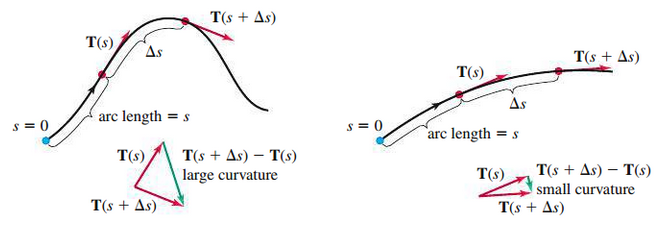
\includegraphics[width=0.8\linewidth]{images/briggs_14_05/fig14_29}
  \end{center}
  \vspace*{\stretch{1}}

  \begin{defn*}[Curvature]
    Let $\vecr$ describe a smooth parameterized curve. If $s$ denotes arc length and $\mathbf T=\vecr'/\abs{\vecr'}$ is the unit tangent vector, the \textbf{curvature} is $\ds\kappa(s)=\abs{\frac{d\mathbf T}{ds}}$.
  \end{defn*}
  \pagebreak

  \noindent
  \fbox{\parbox{0.9875\linewidth}{
    \textbf{Theorem 14.4: Curvature Formula}\\
    Let $\vecr(t)$ describe a smooth parameterized curve, where $t$ is any parameter. If $\vecv=\vecr'$ is the velocity and $\mathbf T$ is the unit tangent vector, then the curvature is
      \[\kappa(t)=\frac{1}{\abs{\vecv}}\abs{\frac{d\mathbf T}{dt}}=\frac{\abs{\mathbf T'(t)}}{\abs{\vecr'(t)}}.\]
  }}
  \begin{itemize}
    \item 
      $\kappa$ is a non-negative scalar-valued function
    \item 
      Curvature of zero corresponds to a straight line
    \item 
      A relatively flat curve has a small curvature
    \item 
      A tight curve has a larger curvature
  \end{itemize}

  \begin{ex*}
    Consider the line
      \[\vecr(t)=\bracket{x_0+at,\,y_0+bt,\,z_0+ct},\textnormal{ for }-\infty<t<\infty.\]
    Compute $\kappa$.
  \end{ex*}

  \pagebreak

  \begin{ex*}
    Consider the circle
      \[\vecr(t)=\bracket{R\cos(t),\,R\sin(t)}\]
    for $0\leq t\leq 2\pi$, where $R>0$. Show that $\kappa=1/R$.
  \end{ex*}
  \vspace*{\stretch{1}}

  \begin{ex*}
    Consider the curve
      \[\vecr(t)=\bracket{2\cos(t),\,2\sin(t),\,\sqrt{5}t}\]
    Compute $\kappa$.
  \end{ex*}
  \vspace*{\stretch{1}}

  \pagebreak
  \textbf{An Alternative Curvature Formula:}\\
  Consider a smooth function $\vecr(t)$ with non-zero velocity $\vecv(t)=\vecr'(t)$ and non-zero acceleration $\mathbf a(t)=\vecv'(t)$. 
    \[\mathbf T=\frac{\vecv}{\abs{\vecv}}\ \Rightarrow\   \vecv=\abs{\vecv}\,\mathbf T.\]
  Thus
    \[\mathbf a=\frac{d\vecv}{dt}=\ddt\sbrkt{\abs{\vecv}\,\mathbf T}=\ddt\sbrkt{\abs{\vecv}}\,\mathbf T+\abs{\vecv}\,\frac{d\mathbf T}{dt}.\]
  Now we form $\vecv\times\mathbf a$:
  \begin{align*}
    \vecv\times\mathbf a&=\abs{\vecv}\,\mathbf T\times\parens{\ddt\sbrkt{\abs{\vecv}}\,\mathbf T+\abs{\vecv}\,\frac{d\mathbf T}{dt}}\\[5pt]
      &=\underbrace{\abs{\vecv}\,\mathbf T\times\ddt\sbrkt{\abs{\vecv}}\,\mathbf T}_{\bfO}+\abs{\vecv}\,\mathbf T\times\abs{\vecv}\,\frac{d\mathbf T}{dt}
  \end{align*}
  Since $\mathbf T$ is a unit vector, $\mathbf T$ and $d\mathbf T/dt$ are orthogonal (Theorem 14.2). Thus
  \begin{align*}
    \abs{\vecv\times\mathbf a}=\abs{\abs{\vecv}\,\mathbf T\times\abs{\vecv}\,\frac{d\mathbf T}{dt}}=\abs{\vecv}\underbrace{\abs{\mathbf T}}_1\,\abs{\abs{\vecv}\frac{d\mathbf T}{dt}}\underbrace{\sin\theta}_1
      =\abs{\vecv}^2 \abs{\frac{d\mathbf T}{dt}}
  \end{align*}
  Now, using Theorem 14.4, where $\ds\abs{\frac{d\mathbf T}{dt}}=\kappa \abs{\vecv}$, we have
    \[\abs{\vecv\times\mathbf a}=\abs{\vecv}^2\abs{\frac{d\mathbf T}{dt}}=\abs{\vecv}^2\,\kappa\abs{\vecv}=\kappa\abs{\vecv}^3.\]

  \vspace*{\stretch{1}}
  \noindent
  \fbox{\parbox{0.9875\linewidth}{
    \textbf{Theorem 14.5: Alternative Curvature Formula}\\
    Let $\vecr$ be the position of an object moving on a smooth curve. The \textbf{curvature} at a point on the curve is
      \[\kappa=\frac{\abs{\vecv\times\mathbf a}}{\abs{\vecv}^3},\]
    where $\vecv=\vecr'$ is the velocity and $\mathbf a=\vecv'$ is the acceleration.
  }}

  \pagebreak

  \begin{ex*}
    Consider the curve
      \[\vecr(t)=\bracket{-16\cos(t),\,16\sin(t),\,0}.\]
    Compute the curvature $\kappa$ using both methods.
  \end{ex*}

  \pagebreak
  \textbf{Principal Unit Normal Vector}\\
  Curvature indicates how quickly a curve turns. The principal unit normal vector determines the \textit{direction} in which a curve turns.

  \begin{defn*}[Principal Unit Normal Vector]
    Let $\vecr$ describe a smooth curve parameterized by arc length. The \textbf{principal unit normal vector} at a point $P$ on the curve at which $\kappa\neq 0$ is
      \[\mathbf N(s)=\frac{d\mathbf T/ds}{\abs{d\mathbf T/ds}}=\frac{1}{\kappa}\frac{d\mathbf T}{ds}.\]
    For other parameters, we use the equivalent formula
      \[\mathbf N(t)=\frac{d\mathbf T/dt}{\abs{d\mathbf T/dt}},\]
    evaluated at the value of $t$ corresponding to $P$.
  \end{defn*}
  \begin{center}
    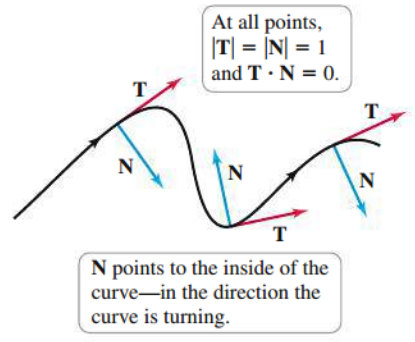
\includegraphics[width=0.275\linewidth]{images/briggs_14_05/fig14_31}
  \end{center}

  \noindent
  \fbox{\parbox{0.9875\linewidth}{
    \textbf{Theorem 14.6: Properties of the Principal Unit Normal Vector}\\
    Let $\vecr$ describe a smooth parameterized curve with unit tangent vector $\mathbf T$ and principal unit normal vector $\mathbf N$.
    \begin{enumerate}
      \item 
        $\mathbf T$ and $\mathbf N$ are orthogonal at all points of the curve; that is, $\mathbf T\cdot\mathbf N=0$ at all points where $\mathbf N$ is defined.
      \item 
        The principal unit normal vector points to the inside of the curve -- in the direction that the curve is turning.
    \end{enumerate}
  }}
  \pagebreak

  \begin{ex*}
    For the curve $\vecr(t)=\bracket{a\cos(t),\,a\cos(t),\,bt}$, find the unit tangent vector $\mathbf T$ and the principal unit normal vector $\mathbf N$. Verify $\abs{\mathbf T}=\abs{\mathbf N}=1$ and $\mathbf T\cdot\mathbf N=0$.
  \end{ex*}

  \pagebreak

  \textbf{Components of the Acceleration}\\
  Recall that the change in velocity, or acceleration, of an object change change in \textit{speed} and in \textit{direction}. 
  
  \noindent
  \fbox{\parbox{0.9875\linewidth}{
    \textbf{Theorem 14.7: Tangential and Normal Components of the Acceleration}\\
    The acceleration vector of an object moving in space along a smooth curve has the following representation in terms of its \textbf{tangential component} $a_T$ (in the direction of $\mathbf T$) and its \textbf{normal component} $a_N$ (in the direction of $\mathbf N$):
      \[\mathbf a=a_N\mathbf N+a_T\mathbf T,\]
    where $a_N=\kappa\abs{\vecv}^2=\ds\frac{\abs{\vecv\times\mathbf a}}{\abs{\vecv}}$ and $a_T=\ds\frac{d^2s}{dt^2}$.
  }}
  \vspace*{\stretch{1}}
  \pagebreak

  \begin{defn*}[Unit Binormal Vector and Torsion]
    Let $C$ be a smooth parameterized curve with unit tangent and principal unit normal vectors $\mathbf T$ and $\mathbf N$, respectively. Then at each point of the curve at which the curvature is nonzero, the \textbf{unit binomial vector} is
      \[\mathbf B=\mathbf T\times\mathbf N,\]
    and the \textbf{torsion} is
      \[\tau=-\frac{d\mathbf B}{ds}\cdot\mathbf N\]
  \end{defn*}

  \noindent
  \fbox{\parbox{0.9875\linewidth}{
    \textbf{Summary: Formula for Curves in Space}\\
    
  }}

  \pagebreak
  
\end{document}